% This is samplepaper.tex, a sample chapter demonstrating the
% LLNCS macro package for Springer Computer Science proceedings;
% Version 2.20 of 2017/10/04
%
\documentclass[runningheads]{llncs}
\newcommand{\quotes}[1]{``#1''}
\newcommand{\singlequotes}[1]{`#1'}
\renewcommand{\arraystretch}{1.5}
%
\usepackage{graphicx}
\usepackage[super]{nth}
\usepackage{mdframed}
\usepackage[most]{tcolorbox}
\usepackage{boldline} 
\usepackage[ruled,vlined]{algorithm2e}
\usepackage{mathtools}
\usepackage{algorithmic}
\usepackage{multicol}
\usepackage{verbatim}
\usepackage[colorinlistoftodos]{todonotes}
\usepackage[ruled]{algorithm2e}


\usepackage{hyperref}
\usepackage{comment}
\usepackage{amsmath,amssymb,amsfonts,amsthm}
\usepackage{mathcomp}

\renewcommand{\algorithmicrequire}{\textbf{Input:}}
\renewcommand{\algorithmicensure}{\textbf{Output:}}



\newtcolorbox[blend into=figures]{myfigure}[2][]{float=htb,
title={#2},#1}
% Used for displaying a sample figure. If possible, figure files should
% be included in EPS format.
%
% If you use the hyperref package, please uncomment the following line
% to display URLs in blue roman font according to Springer's eBook style:
% \renewcommand\UrlFont{\color{blue}\rmfamily}

\begin{document}
%
\title{Password Generation Using Bi-Directional Generative Adversarial Network\\ \quotes{BIPASSGAN}}
%
%\titlerunning{Abbreviated paper title}
% If the paper title is too long for the running head, you can set
% an abbreviated paper title here
%
\author{First Author\inst{1}\orcidID{0000-1111-2222-3333} \and
Second Author\inst{2,3}\orcidID{1111-2222-3333-4444} \and
Third Author\inst{3}\orcidID{2222--3333-4444-5555}}
%
\authorrunning{F. Author et al.}
\titlerunning{BIPASSGAN}
% First names are abbreviated in the running head.
% If there are more than two authors, 'et al.' is used.
%
\institute{Princeton University, Princeton NJ 08544, USA \and
Springer Heidelberg, Tiergartenstr. 17, 69121 Heidelberg, Germany
\email{lncs@springer.com}\\
\url{http://www.springer.com/gp/computer-science/lncs} \and
ABC Institute, Rupert-Karls-University Heidelberg, Heidelberg, Germany\\
\email{\{abc,lncs\}@uni-heidelberg.de}}
%
\maketitle              % typeset the header of the contribution
%
\begin{abstract}
The password is the most prevalent and reliant mode of authentication by date. Recent advancements in IoT have propelled various other mechanisms, but they face severe issues of hardware and software constraints. These scenarios make users rely on this old password-based authentication technique. In the age of no-privacy, human creativity has reached a limit. Passwords used and generated are not secure enough. Deep networks and adversarial created samples are mimicking the unthinkable. The overuse of social networks has exposed our user profiles, which increases risk based on individuals and demands personalized models. We have proposed a novel deep learning approach using a bi-directional generative adversarial network  \quotes{BIPASSGAN} to generate personalized passwords that may be at risk. We have used One-class SVM for determining the strength of the same.

\keywords{Password  \and Machine Learning \and Transfer Learning \and Deep Learning \and GAN \and PASSGAN \and BIGAN \and One-Class SVM}
\end{abstract}
%
%
%
\section{Introduction}
Passwords have been the primary source of authentication since we entered the digital age. After a long technological evolution and evolution of various other authentication techniques, we still rely on the very same passwords. This over-dependence on passwords requires human efforts and creativity for generating new ones and keeping them secure at the same time. In this machine learning and data-centric era, we often talk that privacy is a myth. With cheap computation and readily available resources, it has become effortless to crack passwords. In this paper, we will discuss the current works for guessing passwords. It introduces requirements beyond human creativity to generate secure passwords. Above all, we have thought about personalizing this scheme. The prevailing models are generalized and may prove strong for one case and weak for the other. Transfer learning can come to rescue, and users can have their personalized models. In sections below, we will briefly explain the literature and compare it with what we proposed.

The above study motivates for designing a new novel approach for generating passwords and very same time checking its performance and strength. So, why the human chosen password is still prevalent. It is easy to implement, and no special hardware is required. Human thinks way different beyond machines. From where passwords come from or generated. Human thinking is getting exposed over the years through excessive use of the internet. Machine and deep learning techniques have become smart enough to match our though. It has brought issues into existence that passwords have become easy to guess. We tend to use the same password as they are hard to remember and difficult to type correctly. It makes the user use the same password every time. It increases the probability of attack. Before the advancement of machine learning and deep learning, state of the art for guessing attacks were brute force and dictionary attack. In brute-force \cite{8400211} the attacker tries all the password combinations. With this attack, guessing a password is guaranteed but not feasible because of the time taken. The other one is the dictionary attack, as the name suggests, the dictionary may be a collection of word lists which are common sources for users to choose mnemonic passwords.\cite{8400211} Researchers enhanced guessing attacks using probabilistic context-free grammar(PCFG).\cite{5207658} It assumes that not all guesses have the same probability of cracking a password. For example, the guess "password12" may be more probable than the guess "P@ssW0rd!23" depending on the password creation policy and user creativity. In 2016, Melicher et al. proposed that neural network models can generate human-created passwords.\cite{197243} Recurrent neural networks can learn from sequences. Researchers use Long short-term memory to avoid gradient vanishing problem. \cite{DBLP:journals/corr/Lipton15} All these machine learning algorithms work well. Still, they all have the same limitations as they can only generate a subset of the password possible. Generative Adversarial Network(GAN) has been widely used in recent years for the generation of new and unseen samples in every corners of research. \cite{goodfellow2014generative} With the help of this generative model (Briland Hitaj, Paolo Gasti, Giuseppe Ateniese, Fernando Perez-Cruz) proposed PASSGAN.\cite{DBLP:journals/corr/abs-1709-00440} GAN takes large no of epochs and hence long time for generating passwords. Bi-Directional GAN is an extension of GAN and performs faster in comparison. \cite{DBLP:journals/corr/DonahueKD16}. In GAN, we find the distribution of the data set P(w). With the help of a generator and discriminator, we try to create a distribution with noise(o), which will be similar to P(w). We faced the problem as it takes a longer time to converge the distribution. So, we used Bi Direction GAN in which by adding one more element, we can converge much faster and get satisfactory results on generating new passwords. Further, We trained a One-class SVM model for checking the strength based on all the passwords generated based on training over existing and generated passwords. And, We emphasis on personalized model training such that it proves efficient for individuals. The remainder of this paper is organized as follows. Section II discusses the Data Preprocessing. Section III discusses the architecture of gan and bi gan. Section IV about our model. Section V discusses the experimental result. Section VI discusses password strength evaluation. Section VII experimental result of strength meter section VIII conclusion and IX with future work.

% =======================================================
% # II. Bckground #
% =======================================================

Many authors have proposed and studied password guessing, generation techniques. Earlier, They used brute-force techniques and lexical grammar for this purpose. With cheap resources available and advancements in deep learning, guesswork became easier. Recent models and works analyzed and emulated human thinking and creativity to generate many similar passwords as we can. Nowadays, more exposed profiles have resulted in frequent targeted attacks. It makes the recent works susceptible, ineffective, and motivates us to study them. Research on human chosen passwords is going on for many years. Many researchers try to learn the pattern of passwords and try to memic passwords generating new or similar kinds of passwords. Researchers used natural processing tools to generate a password. Previous tools include using Markov model \cite{Narayanan:2005:FDA:1102120.1102168} to improve the dictionary-based attack.

\textbf{Markov model:} Markov model is based on the Markov chain rule. Markov chain is a mathematical system in which it transits from one state to another state according to certain probabilistic rules. It has many applications in other forms. In password generation, this model uses the idea of a transition between the characters. For example, if we take the word \singlequotes{Alice}. If we use the Markov model of \nth{3} order then the word is divided into \singlequotes{Al}, \singlequotes{lic}, etc. This idea itself becomes its limitation of this model. As for the better result, we have to check all the possibilities of order of Markov model and choose which order Markov model is the best model. Another limitation is that it reaches a lower converge rate of test passwords while generating the same length password. one another limitation is that it is hard to choose the effective word mangling rules to use for a dictionary attack is a hard task. The improvement of this model omen model\cite{10.1007/978-3-319-15618-7_10} was created and adding ranking of passwords to make the cracking of passwords faster.
Then probabilistic context-free grammar model\cite{5207658} was found.
\newline 
\\
\textbf{Probabilistic context-free grammar model:}
This model is the upgrade model of Markov model In this model, their approach was probabilistic and incorporates available information about the probability distribution of user password. They use probabilistic context-free grammar to model the derivation of the structure of the leaked password.
Their starting assumption is that not all guesses have the same probability of cracking a password. For example, the guess “password12” may be more probable than the guess “P@SSW0rd!23” depending on the password creation policy and user creativity. The goal is to generate guesses in decreasing order of probability to maximize the likelihood of cracking the target passwords within a limited number of guesses. To get the probability of the structure they found the probability of digit string, character string, etc in the corpus and they use the concept of context-free grammar to generate a new password. In this method, they find the structure of the password and assign a probability to the structure. Then the find the consecutive alphabet and find their frequency. After that password is generated. \cite{7098389}.After the generation of the password, it can be used for measuring the strength of the user password. Implementation is fuzzy PSM: A New Password Strength Meter Using Fuzzy Probabilistic Context-Free Grammars which use the concept of the model to predict the strength of the password.\cite{7579775}


 \\
 \newline
 \textbf{Recurrent Neural Network:}
 In the meantime, the neural network researcher tries to use the concept of the neural network to crack the passwords, on this process they created Recurrent Neural Network\cite{197243}.It work well but it was unable a generate new type of password as it has vanishing gradient problem it tends to forget the character before. it is hard to choose the best n-gram split. It was the first neural network approach for cracking the password. But due to the vanishing problem an upgrade type of Recurrent Neural Network known as Long short term memory\cite{DBLP:journals/corr/Lipton15}.For the Chinese password, the neural network uses the help of semantic analysis A hierarchical semantic model is made which is based on semantic analysis and long short term memory, analyze patterns and semantics of leaked Chinese passwords dataset which is a collection of leaked passwords from several websites, excluding CSDN passwords. The CSDN passwords are reserved for model testing. Then we segment passwords into meaningful words and meaningless strings. Their neural network is trained with these segmented passwords.\cite{10.1007/978-981-13-5913-2_6}
 \\
 \newline
 \textbf{Deep Learning:}
 After the emergence of deep learning and then the concept of the Generative Model. The researcher used this type of generative model known as GAN(Generative Adversarial Network)\cite{goodfellow2014generative} to generate a new password.More about gan is describe in preliminaries.
\newline
\\
\textbf{Password Guessing Tools:}The oldest password guessing tools were state of the art password guessing tools.It were of two type (a)brute force attack\cite{8400211} (b) dictionary attack\cite{8400211}.A password attack is of two kinds online or offline attacks. In an offline attack, the attacker obtains the hash of the password of some user and tries to get the password by guessing and checking the million of a password. This is a good example of a brute force attack, as in brute force, the attacker tries all possible passwords until it matched the original password. A drawback of this attack as it takes an ample amount of time, and it required a great amount of storage. Whereas in the dictionary attack, the attacker adds some input with a common password based on some rules. In this attack, the attacker tries to reproduce the approach password choice by adding with new words systematically by applying pre-selected mangling rules. For a dictionary attack to be successful, it requires the original word to be in the attacker's input dictionary, and for the attacker to use the correct word-mangling rule. The main challenge of this tool to make offline password attacks is to generate an ordered list of password guesses p1,p2,p3,p4, and so which match with the original password. we have look on this \cite{7566553} securing password from dictionary attack with character tree . An online attack happens when the attacker uses some API to enter password guess against some account. Narayanan and Shmatikov \cite{Narayanan:2005:FDA:1102120.1102168} use Markov models to generate probable passwords. In Password Cracking Using Probabilistic Context-Free Grammars \cite{5207658} they assumed that not all guesses have the same probability of cracking a password. For example, the guess "password12" may be more probable than the guess \quotes{P@ssW0rd!23} depending on the password creation policy and user creativity. In 2016, Melicher et al. proposed that neural networks could model human-created passwords and they used neural networks in password strength measure.\cite{197243}Best a neural network model for sequence text is Recurrent neural networks as it can learn from the sequence. In this model, each password is split ed in n-gram(best result when n=3)
then the n-gram split data is forwarded to the recurrent neural network and a new password is generated but this model has an issue of gradient vanishing problem. To overcome this gradient vanishing problem recurrent neural network is replaced by long short term memory \cite{DBLP:journals/corr/Lipton15}. After the neural network approach came the deep learning approach which is the generative adversarial network(GAN)\cite{goodfellow2014generative}. It is consists of two types of neural network (a) Generator (b) Discriminator which compete with each other. The main idea behind GAN is real data(w) distribution is \textbf{${P_W(w)}$}~ will be given with generated data(u) \textbf{${P_U(u)}$}~from the generator to the discriminator and the discriminator tell whether the data is real or fake and get feedback to generator and generator to try to minimize the error and try to make the distribution similar so that its generated data cannot be discriminated by the discriminator.
\textbf{\[ \minG  \maxD  V (D, G)=E _{w \sim pdata(w)}[log D(w)] + E _{u \sim p u(u)} [log(1-D(G(u)))]. \]}

% =============================================
% # III. Preliminaries #
% =============================================

\section{Data Preprocessing}
The data we have used to generate a new password is the leaked RockYou data set. We have taken a 10,00,000 password. we splitted the data in 80 percent for training and the remaining 20 percent for testing.
\newline
\hfill \break
\textbf{Data cleaning:}~Many data in the data set are still in the hash value. Many passwords are repeated and many are contain non-ASCII characters. We have to remove the non-ASCII character from the data set. Their many passwords of the length of 4 characters. We have taken the mini mun password size 6 and the maximum password of 14 characters. The most common password around a 60 percent password contains lower case letters.
\newline
\hfill \break
\textbf{Data conversion:}~As we split the data set into two-part (a) Training (b) Testing. We take the training data and convert it into an image of the 7*maximum size of the password. To make the dimension of all images the same we set maximum size as 14 by padding space.First we have taken all the number(0-9),upper case character(A,B,..Z),lowercase character(a,b,c,..,z) and special character(@,+,-,&..) total 92 including space.Assign every character of the password with a number. Then we have taken each character from a password and take it decimal representative and convert it into a 7-bit binary representation. We have done this work for all the passwords in the training set.

\section{Architecture Of GAN AND BIGAN}
{\subsection{Generative Adversial Network: }
In this section, we will discuss the generative model. Generative Adversarial Network has been recently introduced to train a generative model to generated new data. It consists of two adversarial networks : (a) Generative model G that captures data distribution, and (b) Discriminative model D that estimate the probability that sample have come from training data or generative model. Both G and D could be multi-level perceptron. In Generative adversarial network generator and discriminator play thief and police game where the generator model tries to fool the discriminator and the discriminator try to discriminate. Initially, the discriminator discriminates easily but as the round increases generator network started to update its parameter.
\\
\begin{figure}[h]
\centering

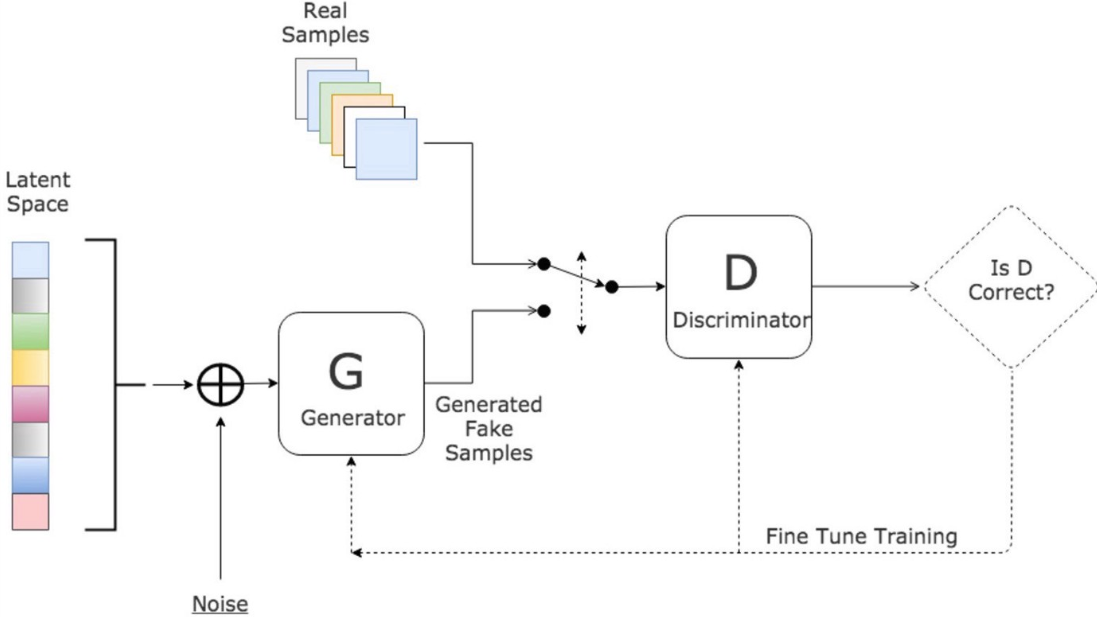
\includegraphics[width=3.5in]{GAN.png}

\caption{GAN}
\label{LP}
\end{figure}

\hfill \break
\textbf{Components of Generative Adversial Network}
\hfill \break
\textbf{Generator Model :}~The main motive of this model is to generate the input distribution as real as possible. Eg-if we take an image from the data set this model to try to learn so that it creates a realistic image of real data.
\hfill \break
\newline
\textbf{Discriminate Model :}~The main motive of this model is to identify the fake image produced by the generator from the real data.
\newline
\hfill \break
\subsection{Working Principle of GAN and k is the least expensive option}
\begin{algorithm*}[H]
%\hspace{-0.5 cm}
%\centering
\caption{Setup}
\label{algo:pre}
%\begin{multicols}{2}
%\underline{{\footnotesize \textbf{Sender's Payment Routine:}}}
%\vspace{-0.4 cm}
\begin{algorithmic}[1]
%\REQUIRE ($S \rightarrow u_1 \rightarrow \cdots \rightarrow u_i \rightarrow \cdots \rightarrow u_n \rightarrow R$, $v$)
%\ENSURE
%\vspace{0.2 cm}
    
    \FOR{$\emph{~no of training iteration} $}
         \FOR{$\emph{k steps}$}
            \STATE \emph{sample m noise sample from noise prior{$P_U(u)$}}
            \STATE \emph{sample m example from data  {$pdata(w)$}}
            \STATE \emph{update the discriminator by ascending its stochastic gradient}
        \ENDFOR
        \STATE \emph{sample m noise sample from noise prior ${P_U(u)}$}
        \STATE \emph{update the generatorby its stochastic gradient}
    \ENDFOR
    \STATE \emph{the gradient based updates can use gradient based learning rule}

 \caption{Algorithm of GAN and k is the least expensive option}    
\end{algorithmic}
%\end{multicols}
%\vspace{-0.3 cm}
\end{algorithm*}

\hfill \break
\subsection{Mathematical Expression of Gan}
\textbf{GAN`s Objective function:}
\newline
\hfill \break
Lets us  assume \textbf{o} refers to \textbf{Noise vector} , \textbf{G(o)} refers to \textbf{Generator output},
\textbf{w} refers to \textbf{training sample} ,
\textbf{D(w)} refers to  Discriminator~ output~ for~ real ~(0,1) ,
\textbf{D(G(o))} refers to  Discriminator~ output~ for~ fake ~(0,1). 
\textbf{At Discriminator: }the main objective is to maximized
\textbf{D(w)}and minimized \textbf{D(G(o))}.where as \textbf{at generator} we want to maximized \textbf{D(G(o))}.Now lets look at the loss function at generator and discriminator.Let look \textbf{at Discriminator D:} \textbf{Dloss_{real}} = log(D(w)) ~~ and Dloss_{fake}=log(1-D(G(o))). ~ So ~the~ \textbf{total~ loss ~is}~ Dloss=Dloss_{real}+Dloss_{fake}~
=~log(D(w))+log(1-D(G(o))) ~ \textbf{the total cost is} 
\newline
    
\begin{equation}
\frac{1}{m} \sum_{i=1}^{m} \log \left(D\left(w^{i}\right)\right)+\log \left(1-D\left(G\left(o^{i}\right)\right)\right)
\end{equation}

\newline
\newline
\hfill \break
\textbf{At Generator G:} ~ \textbf{Gloss=log(1-(D(o)))} ~ or ~\textbf{-log(D(G(o)))}.~\textbf{The total cost is} 
\newline
\hfill

\begin{equation}
\frac{1}{m} \sum_{i=1}^{m} \log \left(1-\left(D\left(o^{i}\right)\right)\right) \quad \text { or } \quad \frac{1}{m} \sum_{i=1}^{m}-\log \left(D\left(G^{i}\right)\right)
\end{equation}

\hfill \break
\newline
\textbf{Total Loss of GAN :} 
\begin{equation}
V(D, G)=E_{w \sim p d a t a(w)}[\log D(w)]+E_{o \sim p o(o)}[\log (1-D(G(o)))]
\end{equation}

\hfill \break
\subsection{ Bi Directional GAN}
Bi-directional GAN just extends the GAN by adding the third component. The third component is the encoder. the work of the encoder is to map the data from data space w to latent space o.the objective of the generator remains the same whereas the objective of the discriminator is altered to classify between the real sample and the fake sample and additionally between a real encoding and a fake encoding.
\\
\begin{figure}[h]
\centering

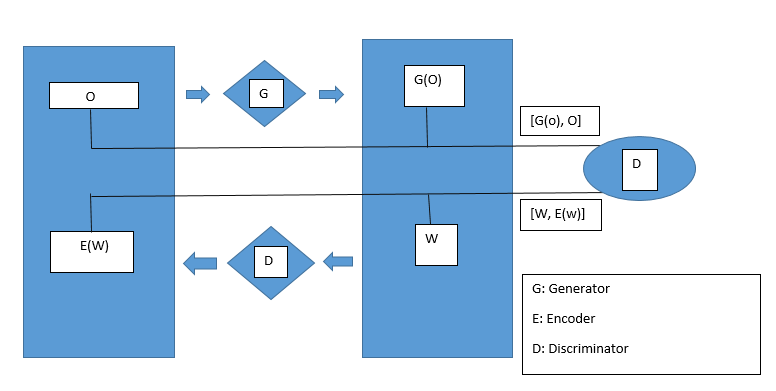
\includegraphics[width=3.5in]{bigan.png}

\caption{BIGAN}
\label{LP}
\end{figure}
\newline

\newline
\hfill \break
\subsection{Components of Bi Directional GAN}
\textbf{Generator(Decoder):}~ Assume that we have a prior belief on where the latent space o lies: $P_{O}(o)$. Given a draw from this latent space the generator G, a deep learner, outputs a synthetic sample is $ {G(o|\theta_G):o}$ is $w_{synthetic}$.Now look at 
\textbf{Encoder:}~~This is the inverse of the generator. From a given data space the encoder E outputs a real encoding. $E(w|\theta_E):w$  is o.\textbf{Discriminator:}~The discriminator classify if a sample is from the real data distribution is ${P_W(w)}$ or the synthetic data distribution $P_G(w|o)$ or classify whether an encoding is real $ P_E(o|w)$  or synthetic $P_O(o) $

\subsection{Working Principle of BiGAN}
\begin{algorithm*}[H]
%\hspace{-0.5 cm}
%\centering
\caption{Setup}
\label{algo:pre}
%\begin{multicols}{2}
%\underline{{\footnotesize \textbf{Sender's Payment Routine:}}}
%\vspace{-0.4 cm}
\begin{algorithmic}[1]
%\REQUIRE ($S \rightarrow u_1 \rightarrow \cdots \rightarrow u_i \rightarrow \cdots \rightarrow u_n \rightarrow R$, $v$)
%\ENSURE
%\vspace{0.2 cm}
    
    \FOR{$\emph{~no of training iteration} $}
         \FOR{$\emph{k steps}$}
            \STATE \emph{Some noise is chosen from random distribution}
            \STATE \emph{That noise is given to the generator to generate data
 and also given to decoder to generate synthetic encoding.}
            \STATE \emph{Real data is given to the encoder for generate real encoding.}
            \STATE \emph{All the four element are given to the discriminator to classify between a real sample and a synthetic sample and additionally between a real encoding and synthetic encoding.
 }
            \STATE \emph{update the discriminator by ascending its stochastic gradient}
        \ENDFOR
        \STATE \emph{sample m noise sample from noise prior ${P_U(u)}$}
        \STATE \emph{update the generator by its stochastic gradient}
    \ENDFOR
    
 \caption{Algorithm of BIGAN}    
\end{algorithmic}
%\end{multicols}
%\vspace{-0.3 cm}
\end{algorithm*}
\hfill \break
\textbf{BIGAN Objective Function:}

\begin{equation}
\begin{array}{c}
{\min _{G\left(o ; \theta_{C}\right), E\left(w ; \theta_{R}\right) D\left[\left(w, \theta_{R}\right) D\left[(w, o) ; \theta_{D}\right]\right.} V\left(D\left[(w, o): \theta_{D}\right], G\left(o ; \theta_{G}\right), E\left(w ; \theta_{E}\right)=\right.} \\
{E_{w \sim P_{W}(w)} E_{o \sim P_{E}(o / w)} \log \left[D\left[(w, o) ; \theta_{D}\right]\right]+} \\
{E_{o \sim P o(o) E_{\mathcal{M}}, P_{a}(\mathcal{L} / o)} \log \left[1-D\left[(\hat{w}, o) ; \theta_{D}\right]\right]}
\end{array}
\end{equation}

\par
\section{Proposed model and creating password }
\subsection{Overview of Our Model}
\newline
\textbf{BIPASSGAN: }We trained our Bigan model with the password data set which we have converted into an image with a dimension of 7*maximum size of the password i.e 14 in our case. We converted each password into an image. Then with the help of encoder, we encoded the image.
Noise from random distribution is taken and with the decoder synthetic encoding. Now all the four things feed to the discriminator to classify between a real sample and a synthetic sample and additionally between a real encoding, i.e., given by the encoder, and a synthetic encoding, i.e., a sample from the latent space. After a certain amount of epoch we able to generate new images that we convert it back to the character, and generate a new password. We have done this experiment in the ubuntu cluster of 30 TB of the hard disk. It took nearly 6 hrs to train the model on the RockYou data set with batch size 64. For optimization, we have chosen Adam Optimizer with a value of 0.002.


\subsection{Working Principle of BIPASSGAN}
\begin{algorithm*}[H]
%\hspace{-0.5 cm}
%\centering
\caption{Setup}
\label{algo:pre}
%\begin{multicols}{2}
%\underline{{\footnotesize \textbf{Sender's Payment Routine:}}}
%\vspace{-0.4 cm}
\begin{algorithmic}[1]
%\REQUIRE ($S \rightarrow u_1 \rightarrow \cdots \rightarrow u_i \rightarrow \cdots \rightarrow u_n \rightarrow R$, $v$)
%\ENSURE
%\vspace{0.2 cm}
    \STATE \emph{Split the data into training and testing}
    \STATE \emph{Conversion of password to image}
    \FOR{$\emph{~no of training iteration} $}
         \FOR{$\emph{k steps}$}
            \STATE \emph{Some noise is chosen from random distribution}
            \STATE \emph{That noise is given to the generator to generate data
 and also given to decoder to generate synthetic encoding.}
            \STATE \emph{Real data is given to the encoder for generate real encoding.}
            \STATE \emph{All the four element are given to the discriminator to classify between a real sample and a synthetic sample and additionally between a real encoding and synthetic encoding.
 }
            \STATE \emph{update the discriminator by ascending its stochastic gradient}
        \ENDFOR
        \STATE \emph{sample m noise sample from noise prior ${P_U(u)}$}
        \STATE \emph{update the generator by its stochastic gradient}
    \ENDFOR
    \STATE \emph{Generate new image}
    \STATE \emph{convert the images to password}
    \STATE \emph{find the unique password}
    
    
 \caption{BIPASSGAN Algorithm and k is the least expensive option}    
\end{algorithmic}
%\end{multicols}
%\vspace{-0.3 cm}
\end{algorithm*}

\begin{figure}
\centering

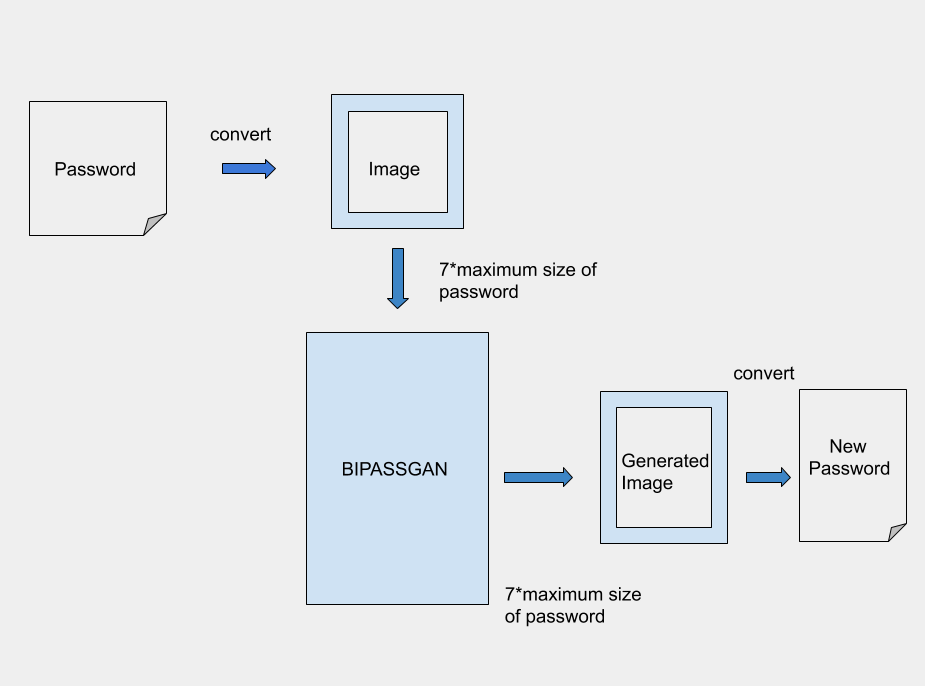
\includegraphics[width=5in]{vc.png}

\caption{BIPASSGAN}
\label{LP}
\end{figure}
\newline

\subsection{Representing Password to Image representation}
\textbf{Conversion: }~ We know that an image is represented in a 2-dimensional array of a pixel. It is easy to element Bi-Directional gan on the image. So we represented each character of the password to 7-bit binary representation so that we can represent a password in a 2-dimensional array. For that, we have taken all the character, numerical, special character and make a dictionary. As we assign a number to each element , whenever we see a character we convert the assigned number to binary. In such a way we create a 2-dimensional array.
\par
\newline
\begin{table}[h]
\centering
\caption{Representing text into binary }
\label{}
\scalebox{0.7}{
\begin{tabular}{||c||c||}
	\hline
	\hline
	\textbf{Password} & \textbf{ Binary Representation} \\
	\hline \hline
    sanjay & '0110110', '0100100', '0110001', '0101101', '0100100', '0111100' \\
	\hline
    sandip & '0110110', '0100100', '0110001', '0100111', '0101100', '0110011' \\
	\hline
	 rockyou  & '0110101', '0110010', '0100110', '0101110', '0111100', '0110010', '0111000' \\

	\hline
	 devil & '0100111', '0101000', '0111001', '0101100', '0101111' \\
    \hline
     passwor & '0110011', '0100100', '0110110', '0110110', '0111010', '0110010', '0110101' \\
     \hline
     Riya & '0011011', '0101100', '0111100', '0100100' \\
    \hline
    123456 & '0000001', '0000010', '0000011', '0000100', '0000101', '0000110' \\
	\hline
	8820337820 &~'0001000', '0001000', '0000010', '0000000', '0000011', '0000011', '0000111', '0001000', '0000010', '0000000'\\
    \hline
    \hline
\end{tabular}}
\end{table}
}

\section{Result}
\subsection{PassGAN Vs Our Model}
\textbf{Evaluating the password: }~After the generation of passwords, with the help of set theory, we can find a unique password generated by the model. First, we take all the test data into a set to find the unique test password. Then we compare the generated password with the test data.we have significant results compared to the first deep learning approach.
\newline

\begin{table}[htb]
\centering
\caption{Result of passgan using the Rockyou data set in 199000 iterations}
\label{}
\scalebox{0.8}{
\begin{tabular}{||c||c||c||}
	\hline
	\hline
	\text{Password Generated} & \text{Unique Password} & \text{Password Matched(1978367 unique sample)}\\
	\hline
	\hline
    10^4 & 9738 & 103(0.005)\\
	\hline
    10^5 & 94400 & 975(0.048)\\
	\hline
	10^6 & 855972 & 7543(0.381)\\
	\hline
	10^7 & 7064483 & 40320(2.038)\\
	\hline
	\hline
\end{tabular}}

\end{table}


\par
\begin{table}[htb]
\centering
\caption{Result of bipassgan using the My space data in 160000 iteration}
\label{}
\scalebox{0.8}{

\begin{tabular}{||c||c||c||}
	\hline
	\hline
	\text{Password Generated} & \text{Unique Password} & \text{Password Matched(145588 unique sample)}\\
	\hline
	\hline
    10^4 & 9878 & 247(0.16)\\
	\hline
    10^5 & 97323 & 112(0.76)\\
	\hline
	10^6 & 971712 & 6234(4.28)\\
	\hline
	10^7 & 8732545 &32571(22.3)\\
	\hline
	\hline
\end{tabular}
}
\end{table}

\par
\newline
\begin{table}[htb]
\centering
\caption{Result of bipassgan using the rockyou data set in 160000 iteration}
\label{}
\scalebox{0.8}{

\begin{tabular}{||c||c||c||}
	\hline
	\hline
	\text{Password Generated} & \text{Unique Password} & \text{Password Matched(145588 unique sample)}\\
	\hline
    10^4 & 9978 & 287(0.18)\\
	\hline
    10^5 & 99473 & 1334(0.87)\\
	\hline
	10^6 & 978976 & 7318(4.78)\\
	\hline
	10^7 & 8324568 &39648(25.8)\\
	\hline
	\hline
\end{tabular}}
\end{table}

\newline
\begin{figure}[ht!] %!t
\centering
\begin{mdframed}
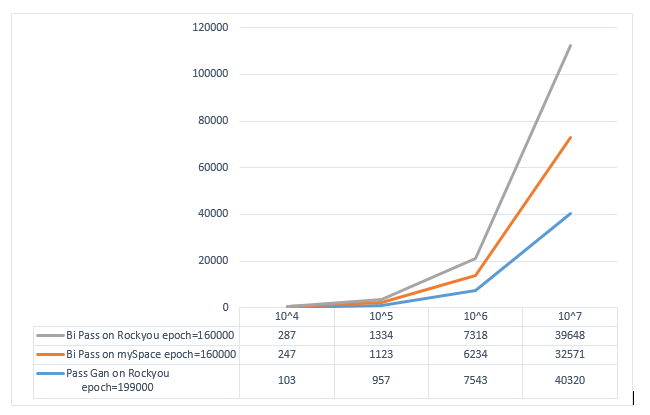
\includegraphics[width=4 in]{Compare.png}
\end{mdframed}
\caption{Compare Between PASSGAN AND BIGAN}
\label{LP}
\end{figure}
\newline


\section{Password Strength Evaluation:}
With the help of one-class SVM, we have evaluated the strength of the password. We have trained the one-class SVM model\cite{1437839} with the generated password that we have generated from the Bigan. After training the model with the password we test it a human-created password and check whether the password is weak, normal or strong.
\newline
\hfill \break
\textbf{Support Vector Machine:} ~Let's take look at the traditional two-class support vector machine(SVM).Consider a data set $Ω={(w1,u1),(w2,u2) ,…,(w_n,u_n)}$\;\\ ~where ~ $w_i$\ is the input data point and $u_i$\ indicate the class. The property of SVM is that it helps in separating data into a class. Datapoint which cannot be separated by a straight line in original space is lifted to higher space where there can be a “straight” hyperplane that separates the data points of one class from another. When that hyperplane would be projected back to the input space, it would have the form of a non-linear curve. It is one of the best algorithms for classification problems. But as we have no label data we unable to use a two-class support vector machine, for this reason, we take the help of a one-class support vector machine.

\par
\newline
\begin{table}[htb]
\centering
\caption{Few example of Feature Extraction for one class SVM }
\label{}
\scalebox{0.8}{

\begin{tabular}{||c||c||c||c||c||c||c||}
	\hline
	\hline
	\text{Password} & \text{char length} & \text{numeric} & \text{alphabet} & \text{specials} & \text{vowel} & \text{consonants} \\
	\hline
	\hline
    password   & 8 & 0&  8&0&2&6\\
	\hline
     boncev  & 6  & 0  &6&0&2&4\\
    \hline
     dWrraq  & 6 &   0&6&0&1&5\\
    \hline
     ojscatgxp &9  &  0&9&0&2&7\\
    \hline
    beoYobs & 7 &  0&7&0&3&4\\
    \hline
     G48gi & 5 &  0&3&0&1&2\\
    \hline
     1aWdWpk" & 8 &  1&6&1&1&5 \\
     \hline
 rpgscqsF & 8 & 0&8&0&0&8\\
 \hline
 ohi!ewg8J & 9 & 1&7&1&3&4\\
 \hline
 NOCD88 & 6&  2&4&0&1&3\\
 \hline
 pqblmiq/ &8 & 0&7&1&1&6\\
 \hline
 wanoe47 & 7 & 2&5&0&3&2\\ 
 \hline
 jikiqa & 6 & 0&6&0&3&3\\
 \hline
 WioY00 & 6 & 2&4&0&2&2\\
 \hline
 qiskn & 5& 0&5&0&1&4\\
 \hline
 
 9uH"8w90 &8 & 4&3&1&1&2\\
 \hline
 qomeccdltX & 10 & 0&10&0&3&7\\
 \hline
 Wnqjrcl & 7 & 0&7&0&0&7\\
 \hline
 iran85 & 6 & 2&4&0&1&3\\
\hline
ambirdf5 & 8 & 1&7&0&2&5\\
\hline
clile!5 & 7 & 1&5&1&1&4\\

	\hline
	\hline
\end{tabular}
}
\end{table}


\newline
\hfill \break
\newline
\textbf{One class support vector machine:}
{~In one-class SVM, the model is trained on data that has only one class that is normal data. It infers the properties of normal cases and with the help of these properties can predict which are unlike the normal example. with the help of this, we have measured the strength of the password. One class SVM consists of outlier and inlier.when we enter a new password for testing for prediction, it returns the score from which we calculate the distance from the outlier and inlier and determine whether the strength of the password.\\
\hfill \break
\textbf{Result:}~First, we have train our SVM model with 70 percent of RockYou leaked password and tested the model with a summation of 30 percent of RockYou and 30 percent of my space. We found that a number of a strong password are 11983(16\% percent), a number of the medium password are 23257(31\% percent), a number of the weak password is 39618(52\% percent).In  \figref{First Experiment }. we have shown some results of our first test and the bar chart.
\newline
In the second we have trained our one-class SVM model with 70 percent of RockYou leaked password and 70 percent of my space leaked password and tested the model with a summation of 30 percent of RockYou and 30 percent of my space. We found that a number of a strong password is 18912(34.47\% percent), the number of the medium password is 16130(29\% percent), the number of the weak password is 19186(34.97\% percent).In  \figref{Second Experiment}. we have shown some results of our second test and the bar chart.
\newline
In the third, we have trained our one-class SVM model with 60 percent of RockYou leaked password and 60 percent of my space leaked password and 60 percent of the generated password by BiGAN and tested the model with a summation of 40 percent of RockYou and 40 percent of my space. We found that the number of a strong password is 7429(21\% percent), the number of the medium password is 4284(12\% percent), number of weak passwords 23524(66\% percent).In \figref{Third Experiment}. we have shown some results of our third test.
\begin{figure}
  \centering
  \begin{minipage}[b]{0.4\textwidth}
  \begin{mdframed}
    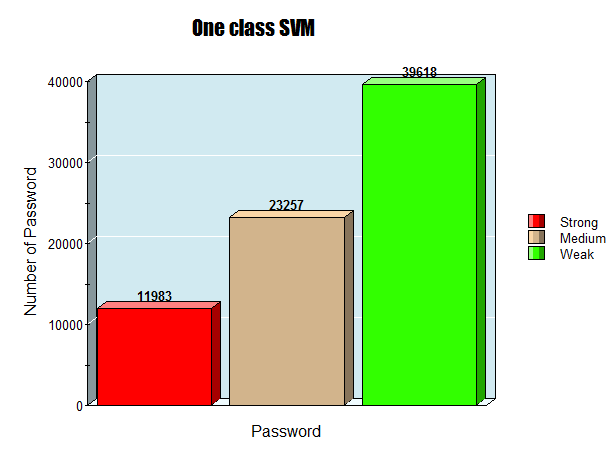
\includegraphics[width=\textwidth]{First.png}
   \end{mdframed}
    \caption{First Experiment.}
  
  \end{minipage}
  
  \hfill
  \centering
  \begin{minipage}[b]{0.4\textwidth}
  \begin{mdframed}
    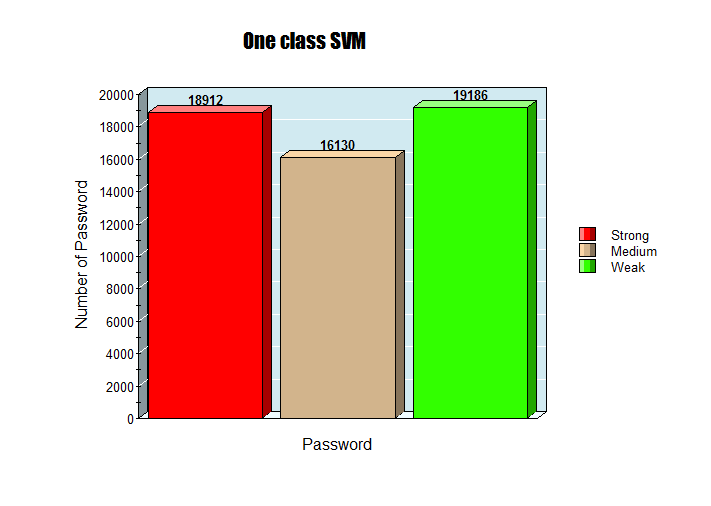
\includegraphics[width=\textwidth]{Secound.png}
\end{mdframed}    
    \caption{Second Experiment.}
  \end{minipage}
  \hfill
  \begin{minipage}[b]{0.4\textwidth}
  \begin{mdframed}
    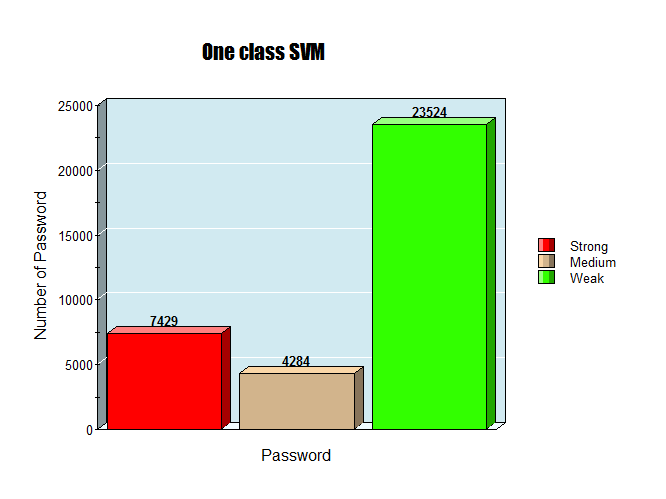
\includegraphics[width=\textwidth]{Third.png}
    \end{mdframed}
    \caption{Third Experiment.}
  \end{minipage}
\end{figure}
\newline
}
\section{Password strength history:}
with the advancement of the neural network, the researcher used the neural network for measuring the strength of the password.\cite{197243}.as we know the password the oldest and still the most frequently used authentication method. A password strength estimator can significantly help the user to choose a strong password. Tools till now are only been tested on the English language and not tested on any other language. In this paper,\cite{article} they have adapted the password strength meter in the Czech language. They have adapted the zxcvbn estimation engine for the Czech and Slovak languages.there is much research going on the policy of password creation. In this paper, \cite{GUO2019423}the researcher has found a password policy known as optiwords which is easy to remember by the user.  Optiwords is a new textual password creation policy that is based on picture superiority effect, which provides users with a direct “drawing-to-text” method for creating user-friendly passwords.Password strength meter depends on the amount of training dataset available in this paper \cite{Guo2018LPSELP} they have proposed a lightweight password strength meter known as LPSE: Lightweight password-strength
estimation. In this model, they make a vector representation of the password and compare their cosine similarity and edit distance between the password. Based on the cosine similarity and edit distance, they have given score. After adding all the score they predict whether the password is weak or strong.



\section{Password Strength Metre:}
{We have created a password strength meter with the help of a one-class support vector machine. with the help of the tool called PARS by Georgia Tech university, we have created a data set of passwords with their strength. We then extracted features from the password. The features are the length of the password, number of vowels, number of special characters, number of the alphabet, number of consonants and number of numerical. We have done two testings with the data set \par 1. In the first experiment we have trained the one-class SVM with 70 percent of data set and test with 30 percent of the data set we got an accuracy of 87 percent but when we added the generated data with data set the accuracy drop to 55 percent it shows that we have successfully created a large subset of unique password
\par
\begin{figure}
  \centering
\begin{minipage}[b]{0.8\textwidth}
  \begin{mdframed}
    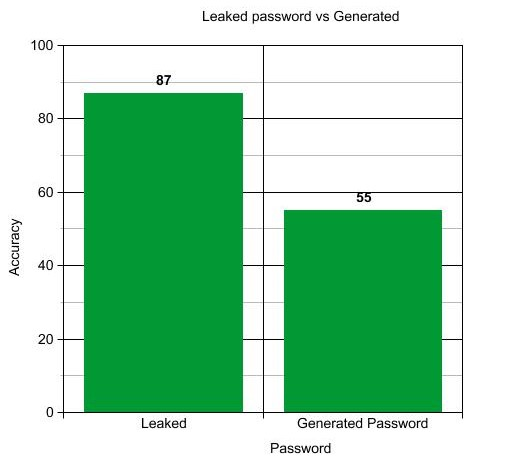
\includegraphics[width=\textwidth]{graph.jpg}
    \end{mdframed}
    \caption{Our Password Strength metre Accuracy}
  \end{minipage}
\end{figure}
\hfill
\par
2. In the second experiment we give the data set to one class for training. And for testing, we are taking input from the password from the user and give the strength of the user input password. By comparing it with the available it showing the great result.
\begin{table}[htb]
\caption{Few example of One class Support Vector Machine Password Strength Checker}
\begin{tabular}{||c||c||c||c||}
	\hline
	\hline
	\textbf{Password} & \textbf{Existing Meter} & \textbf{Our Model}&\textbf{Remarks} \\
	\hline
	
     \$ANju8820   & Very Strong & Weak & name of user \\
 \hline
 Kundan@#1994  & Very Strong  & Good & name and date of birth \\
 \hline
 JAY!@#882037820  & Very Strong & Good & phone no \\
 \hline
 Bhavendra206 & Strong & Good & simple text\\
 \hline
 8963343643 & Weak & Weak & phone no\\
 \hline
 25081998@devil & Strong & Good & simple\\
 \hline
 lucy@!#9863 & Strong & Weak  & nickname\\
 \hline
 Sirdhar123456!@ & Strong & Good& sequence no\\
 \hline
 lovemysoul & Weak & Weak& simple text\\
 \hline
 liveThelife@1231224 & Strong& Strong& random no\\
 \hline
 netdome8752dxja &Strong &Good& simple text\\
 \hline
 amazon2345da & Good & Good& company\\ 
 \hline
 SANjgaydyatig & Good & Strong& random character\\
 \hline
 Riya@199578fdjy & Strong & Good& name\\
 \hline
 juhiGyani@kichkich & Strong& Strong& name\\
 \hline
 Shikhatek+457674 &Strong & Good& name\\
 \hline
 JyotiKhateN1235 & Strong & Good& name\\
 \hline
 PiyaDon45678 & Strong & Medium& name and dictionary word\\
 \hline
 RiyaJay14758788534 & Strong & Strong& random no\\
\hline
Abcjgdjkash & Weak & Good& random character\\
\hline
123456789 & Weak & Weak& sequence of no\\
\hline
987654321 & Weak & Weak&reverse sequence of number\\
\hline
am1AStrongPassword# & Very Strong & strong& dictionary character\\ 
\hline
11@Mushtehara &Very Strong&good& dictionary character\\
\hline
@nebullae&Very Strong&weak& simple text\\
\hline
!ThereisnoHope12!&Strong&strong& character number and special character \\
\hline
Creator@92&Strong&weak& dictionary word\\
\hline
ds101@iitpnitrkl&Very Strong&strong& combination of everything\\
\hline
som735@iitp&Strong&weak& name of the institute\\
\hline
Xiaomi Redmi Airdots&Strong&medium& company names\\
\hline
joinstar1Q!&Strong&medium& meaningful word\\
\hline
Indianlovesindia@9371&Very Strong&strong& long simple text\\
\hline
xp07DY@?1302_&Very strong&medium& gan created\\
\hline
@Enjoy321#&Very strong&weak&sequence no\\
	\hline
	\hline
\end{tabular}

\end{table}
}

\section{Password suggestion}
\textbf{Password Suggestion: }We all want our system more secure but as we choose a common word as our password or some dictionary word with some numerical or special character. These leads to easy cracking of the password. To overcome this we come up with a model that not only checks the strength of the password but also suggests some strong password if the user has chosen a weak password.
\subsection{Overview: }Our model consists of our password strength checker for measuring the strength of the password and BIPASSGAN for generating a new password. The password strength checker model is an extension of the one-class SVM model which we have trained with leaked password as well as the password generated by BIPASSGAN.In this model, we have slightly change the BIPASSGAN in which we have taken the weak password, with the information of the user to train our bigan model. Then it sorts the password with their strength score and gives the user top ten strong password

\begin{figure}
  \centering
\begin{minipage}[b]{0.8\textwidth}
  \begin{mdframed}
    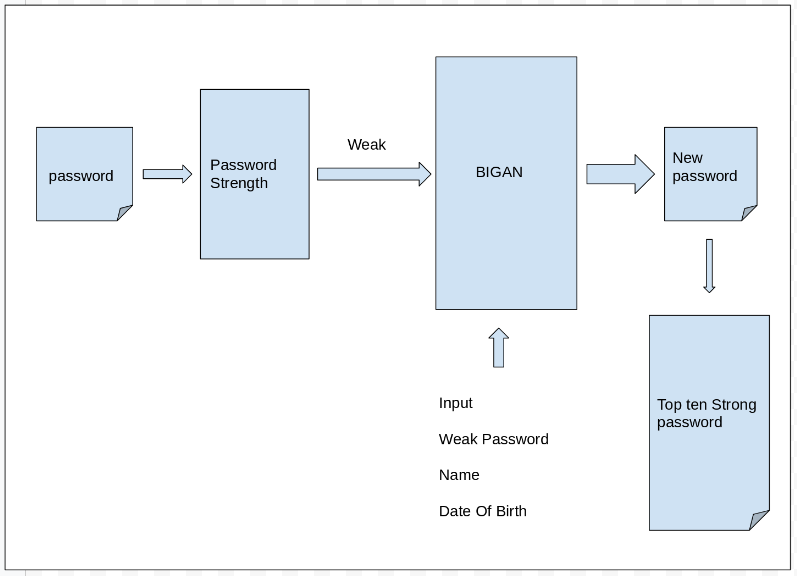
\includegraphics[width=\textwidth]{ab.png}
    \end{mdframed}
    \caption{Our Model}
  \end{minipage}
\end{figure}
\section{Conclusion}

We conclude that though we have pass gan the first deep learning approach for generating a password from the leaked data and we have seen that pass gan has overcome all other generating password technique set but with this new approach \textbf{\quotes{BIPASSGAN}} we have generated a password with less epoch and our generated password is closer to human-created password. So we can conclude that our model is better than pass gan.  We have designed a strength evaluator with the ample amount of passwords generated by bi-pass gan,  that works on the approach of a one-class support vector machine. By comparing it with the available strength meter we have concluded that our strength evaluator surpasses the available strength meter.

\section{Future Works}
We can use the concept of transfer learning for tuning Bidirectional GAN. As we trained the bi gan model with a large dataset and it takes a huge amount of time to complete. So we can use the concept of transfer learning to retrain the gan model whenever the new dataset is given. We have used the one-class SVM model for analyzing the strength of the password. Tuning of one class SVM can be found as it has only one class and it hard to tune the best parameter for the one-class SVM. We can use it for password suggestions. If our one-class SVM predicts that the user password is weak it will suggest other strong passwords for the user.


% ==================
% # IV. CONCLUSION #
% ==================

%
% ---- Bibliography ----
%
% BibTeX users should specify bibliography style 'splncs04'.
% References will then be sorted and formatted in the correct style.
%
% \bibliographystyle{splncs04}
% \bibliography{mybibliography}
%
%\begin{thebibliography}
%\bibliographystyle{splncs04}
%\bibitem{test}
%fdfd
%\end{thebibliography}

\bibliographystyle{IEEEtran}
\bibliography{bibliography.bib}
\end{document}
